A \textbf{Single Nucleotide Polymorphism (SNP)} is a DNA sequence variation occurring commonly within a population (e.g. 1 per cent) in which a Single Nucleotide — A, T, C or G — in the genome differs between members of a biological species or paired chromo-somes. 
\\
\\For example, if we have two sequenced DNA fragments from different individuals (see \emph{Figure 2.1}):

\begin{itemize}
	\item AAGCCTA
	\item AAGCTTA
\end{itemize}

The second one contain a difference in a single nucleotide. In this case we say that there are two alleles. Almost all common SNPs have only two alleles. 

The genomic distribution of SNPs is not homogenous; SNPs occur in non-coding regions more frequently than in coding regions.

\newpage

The main causes of a SNP are:

\begin{enumerate}
	\item natural selection, acting and fixating the allele of the SNP that constitutes the most favorable genetic adaptation
	\item like genetic recombination
	\item mutation rate
	\end{enumerate}

\begin{figure}[ht!]
	\centering
	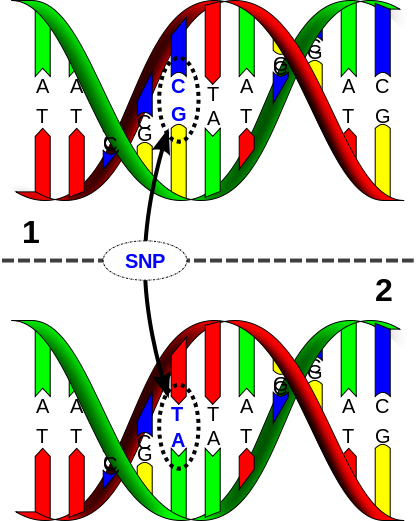
\includegraphics[width=60mm]{../Images/SNP_example.png}
	\label{overflow}
	\caption{SNP example}
	\end{figure}

\section{The different possible types of SNPs}
As previously seen, Single Nucleotide Polymorphisms may fall within \emph{coding} sequences of genes, \emph{non-coding} regions of genes, as well as in the \emph{intergenic} regions (regions between genes).

\subsection{What is a coding?}
To understand the difference between SNPs’ types, we have to see what a coding is.
\\
\\
\\The main concept to analyse is the \textbf{Genetic Code}: it is the \emph{set of rules} by which information encoded within genetic material (DNA or even mRNA sequences) is \emph{translated} into proteins by living cells.
\\
\\
During the translation, the sequence of nitrogenous bases is treated in groups of three at a time; a group of three nitrogenous bases is called a \textbf{codon}. The code defines how codons specify which amino acid will be added next during protein synthesis. Generally, three-nucleotide codon in a nucleic acid sequence specifies a single amino acid. On the other hand, \textbf{a single amino acid can be specified by more than one codon}: this is the key concept that we will need in the following.
\\
\\To understand better, here is the table that shows, for each amino acid (20 in total + START and STOP), the sequences that can generate it:

\begin{tabular}{|l|rl|}
\hline
Amino acid          &		 Codons        &       \\
\hline
Ala/A 		&	GCT, GCC, GCA, GCG       &      	\\
Arg/R 		&	CGT, CGC, CGA, CGG, AGA, AGG       &      		\\
Asn/N	 	&	AAT, AAC       &      	\\
Asp/D		&	GAT, GAC       &      	\\
Cys/C		&	TGT, TGC       &      	\\
Gln/Q		&	CAA, CAG       &      	\\
Glu/E		&	GAA, GAG       &      	\\
Gly/G		&	GGT, GGC, GGA, GGG       &      	\\
His/H		&	CAT, CAC       &      	\\
Ile/I		&	ATT, ATC, ATA       &      	\\
Leu/L		&	TTA, TTG, CTT, CTC, CTA, CTG       &      	\\
Lys/K		&	AAA, AAG       &      	\\
Met/M		&	ATG       &      	\\
Phe/F		&	TTT, TTC       &      	\\
Pro/P		&	CCT, CCC, CCA, CCG       &      	\\
Ser/S		&	TCT, TCC, TCA, TCG, AGT, AGC       &      	\\
Thr/T		&	ACT, ACC, ACA, ACG       &      	\\
Trp/W		&	TGG       &      	\\
Tyr/Y		&	TAT, TAC       &      	\\
Val/V		&	GTT, GTC, GTA, GTG       &      	\\
START		&	ATG       &      	\\
STOP		&	TAA, TGA, TAG       &      	\\
\hline
\end{tabular}

\newpage

\subsection{SNPs in the coding sequences}
SNPs that fall in this category can be divided into two subcategories:

\begin{enumerate}
	\item Synonymous
	\item Nonsynonymous
	\begin{itemize}
	\item Missense
	\item Nonsense
	\end{itemize}
	\end{enumerate}

First ones does not result in a change in the protein sequence, because the “original” sequence and the real sequence of bases both code the same amino acid.
\\
\\Second ones, instead, change the amino acid sequence of protein. In their turn, they can be of two types: \emph{Missense}, in which a single nucleotide change results in a codon that codes for a different amino acid (that can render the resulting protein non-functional), and \emph{Nonsense}, that results in a premature stop codon, or a nonsense codon and then in a truncated, incomplete, and usually non-functional protein product.
\\
\\
\\
\\Let us see an example of \emph{Missense mutation}:
\\
\\Original DNA code for the amino acid sequence:

\vspace{5mm}

\begin{tabular}{|l|l|l|l|l|l|rl|}
\hline
C   A   T         &	C   A   T         &	C   A   T         &	C   A   T         &	C   A   T         &	C   A   T         &	C   A   T  	&       \\
\hline
\end{tabular}

\vspace{15mm}

Resulting amino acids:

\vspace{5mm}

\begin{tabular}{|l|l|l|l|l|l|rl|}
\hline
His         &	His         &	His         &	His         &	His         &	His         &	His  	&       \\
\hline
\end{tabular}

\vspace{25mm}

If we had, for example, a replacement of the eleventh nucleotide:

\vspace{5mm}

\begin{tabular}{|l|l|l|l|l|l|rl|}
\hline
C   A   T         &	C   A   T         &	C   A   T         &	C   \textbf{C}   T         &	C   A   T         &	C   A   T         &	C   A   T  	&       \\
\hline
\end{tabular}

\vspace{15mm}

Resulting amino acids will be:

\vspace{5mm}

\begin{tabular}{|l|l|l|l|l|l|rl|}
\hline
His         &	His         &	His         &	\textbf{Pro}         &	His         &	His         &	His  	&       \\
\hline
\end{tabular}

\vspace{25mm}

This is, instead, an example of \emph{Nonsense mutation}:
\\
\\Original DNA code for the amino acid sequence:

\vspace{5mm}

\begin{tabular}{|l|l|l|l|l|l|rl|}
\hline
A   T   G         &	A   C   T         &	C   A   C         &	C   G   A         &	G   C   G         &	C   G   A         &	A   G   C  	&       \\
\hline
\end{tabular}

\vspace{15mm}

Resulting amino acids:

\vspace{5mm}

\begin{tabular}{|l|l|l|l|l|l|rl|}
\hline
Met         &	Thr         &	His         &	Arg         &	Ala         &	Arg         &	Ser  	&       \\
\hline
\end{tabular}

\vspace{15mm}

If we had, for example, a replacement of the tenth nucleotide:

\vspace{5mm}

\begin{tabular}{|l|l|l|l|l|l|rl|}
\hline
A   T   G         &	A   C   T         &	C   A   C         &	\textbf{T}   G   A         &	G   C   G         &	C   G   A         &	A   G   C  	&       \\
\hline
\end{tabular}

\vspace{15mm}

Resulting amino acids will be:

\vspace{5mm}

\begin{tabular}{|l|l|l|l|l|l|rl|}
\hline
Met         &	Thr         &	His         &	\textbf{Stop}         &	            &	            &	     	&       \\
\hline
\end{tabular}

\vspace{20mm}

Nonsense mutation are jointly responsible for many diseases; they can cause a genetic disease by damaging a gene responsible for a specific protein (for example \emph{dystrophin} in \emph{Duchenne muscular dystrophy}). 
\\
\\Examples of diseases in which nonsense mutations are known to be among the causes include:

\begin{itemize}
	\item \textbf{Cystic fibrosis}
	\item \textbf{Duchenne muscular dystrophy} (dystrophin)
	\item \textbf{Beta thalassaemia} (beta-globin)
	\item \textbf{Hurler syndrome}
	\end{itemize}

\vspace{10mm}

On the other hand, cancer associated Missense mutations can lead to drastic desta-bilisation of the resulting protein.


\subsection{SNPs not in coding regions}

SNPs that are not in protein-coding regions may still affect:

\begin{enumerate}
	\item gene splicing
	\item transcription factor binding
	\item messenger RNA degradation
	\item \ldots
	\end{enumerate}

Gene expression affected by this type of SNP is referred to as an \textbf{eSNP} (\emph{expression SNP}).